\documentclass[10pt, a4paper]{article}
\usepackage{times}
\usepackage{titlesec}
\usepackage{graphicx}
\usepackage{lipsum}
\usepackage[labelformat=empty]{caption}

\titlespacing*{\section}
{-10pt}{0.75\baselineskip}{.55\baselineskip}
\titlespacing*{\subsection}
{-5pt}{.5\baselineskip}{.25\baselineskip}
\titlespacing*{\subsubsection}
{-3pt}{.3\baselineskip}{.1\baselineskip}
\title{Projeto POO\\
        Simulação de Casas Inteligentes}
\author{Bruno Gião a96544 \\ Miguel Vaz a72161 \\ João Cruz a95375 \\ Grupo 1}
\date{UM, LCC, 2021/2022}

\begin{document}
\maketitle
\begin{figure}[!htb]
\begin{minipage}{0.33\textwidth}
        \centering
        
\includegraphics[width=\linewidth]{Bruno.png}
        \caption{Bruno Gião a96544}
\end{minipage}
\begin{minipage}{0.33\textwidth}
        \centering
        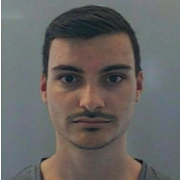
\includegraphics[width=\linewidth]{Joao.png}
        \caption{João Cruz a95375}
\end{minipage}\hfill
\begin{minipage}{0.30\textwidth}
        \centering
        
\includegraphics[width=\linewidth]{Miguel.png}
        \caption{Miguel Vaz a72161}
\end{minipage}
\end{figure}
\newpage
\tableofcontents
\begin{figure}
        \centering
        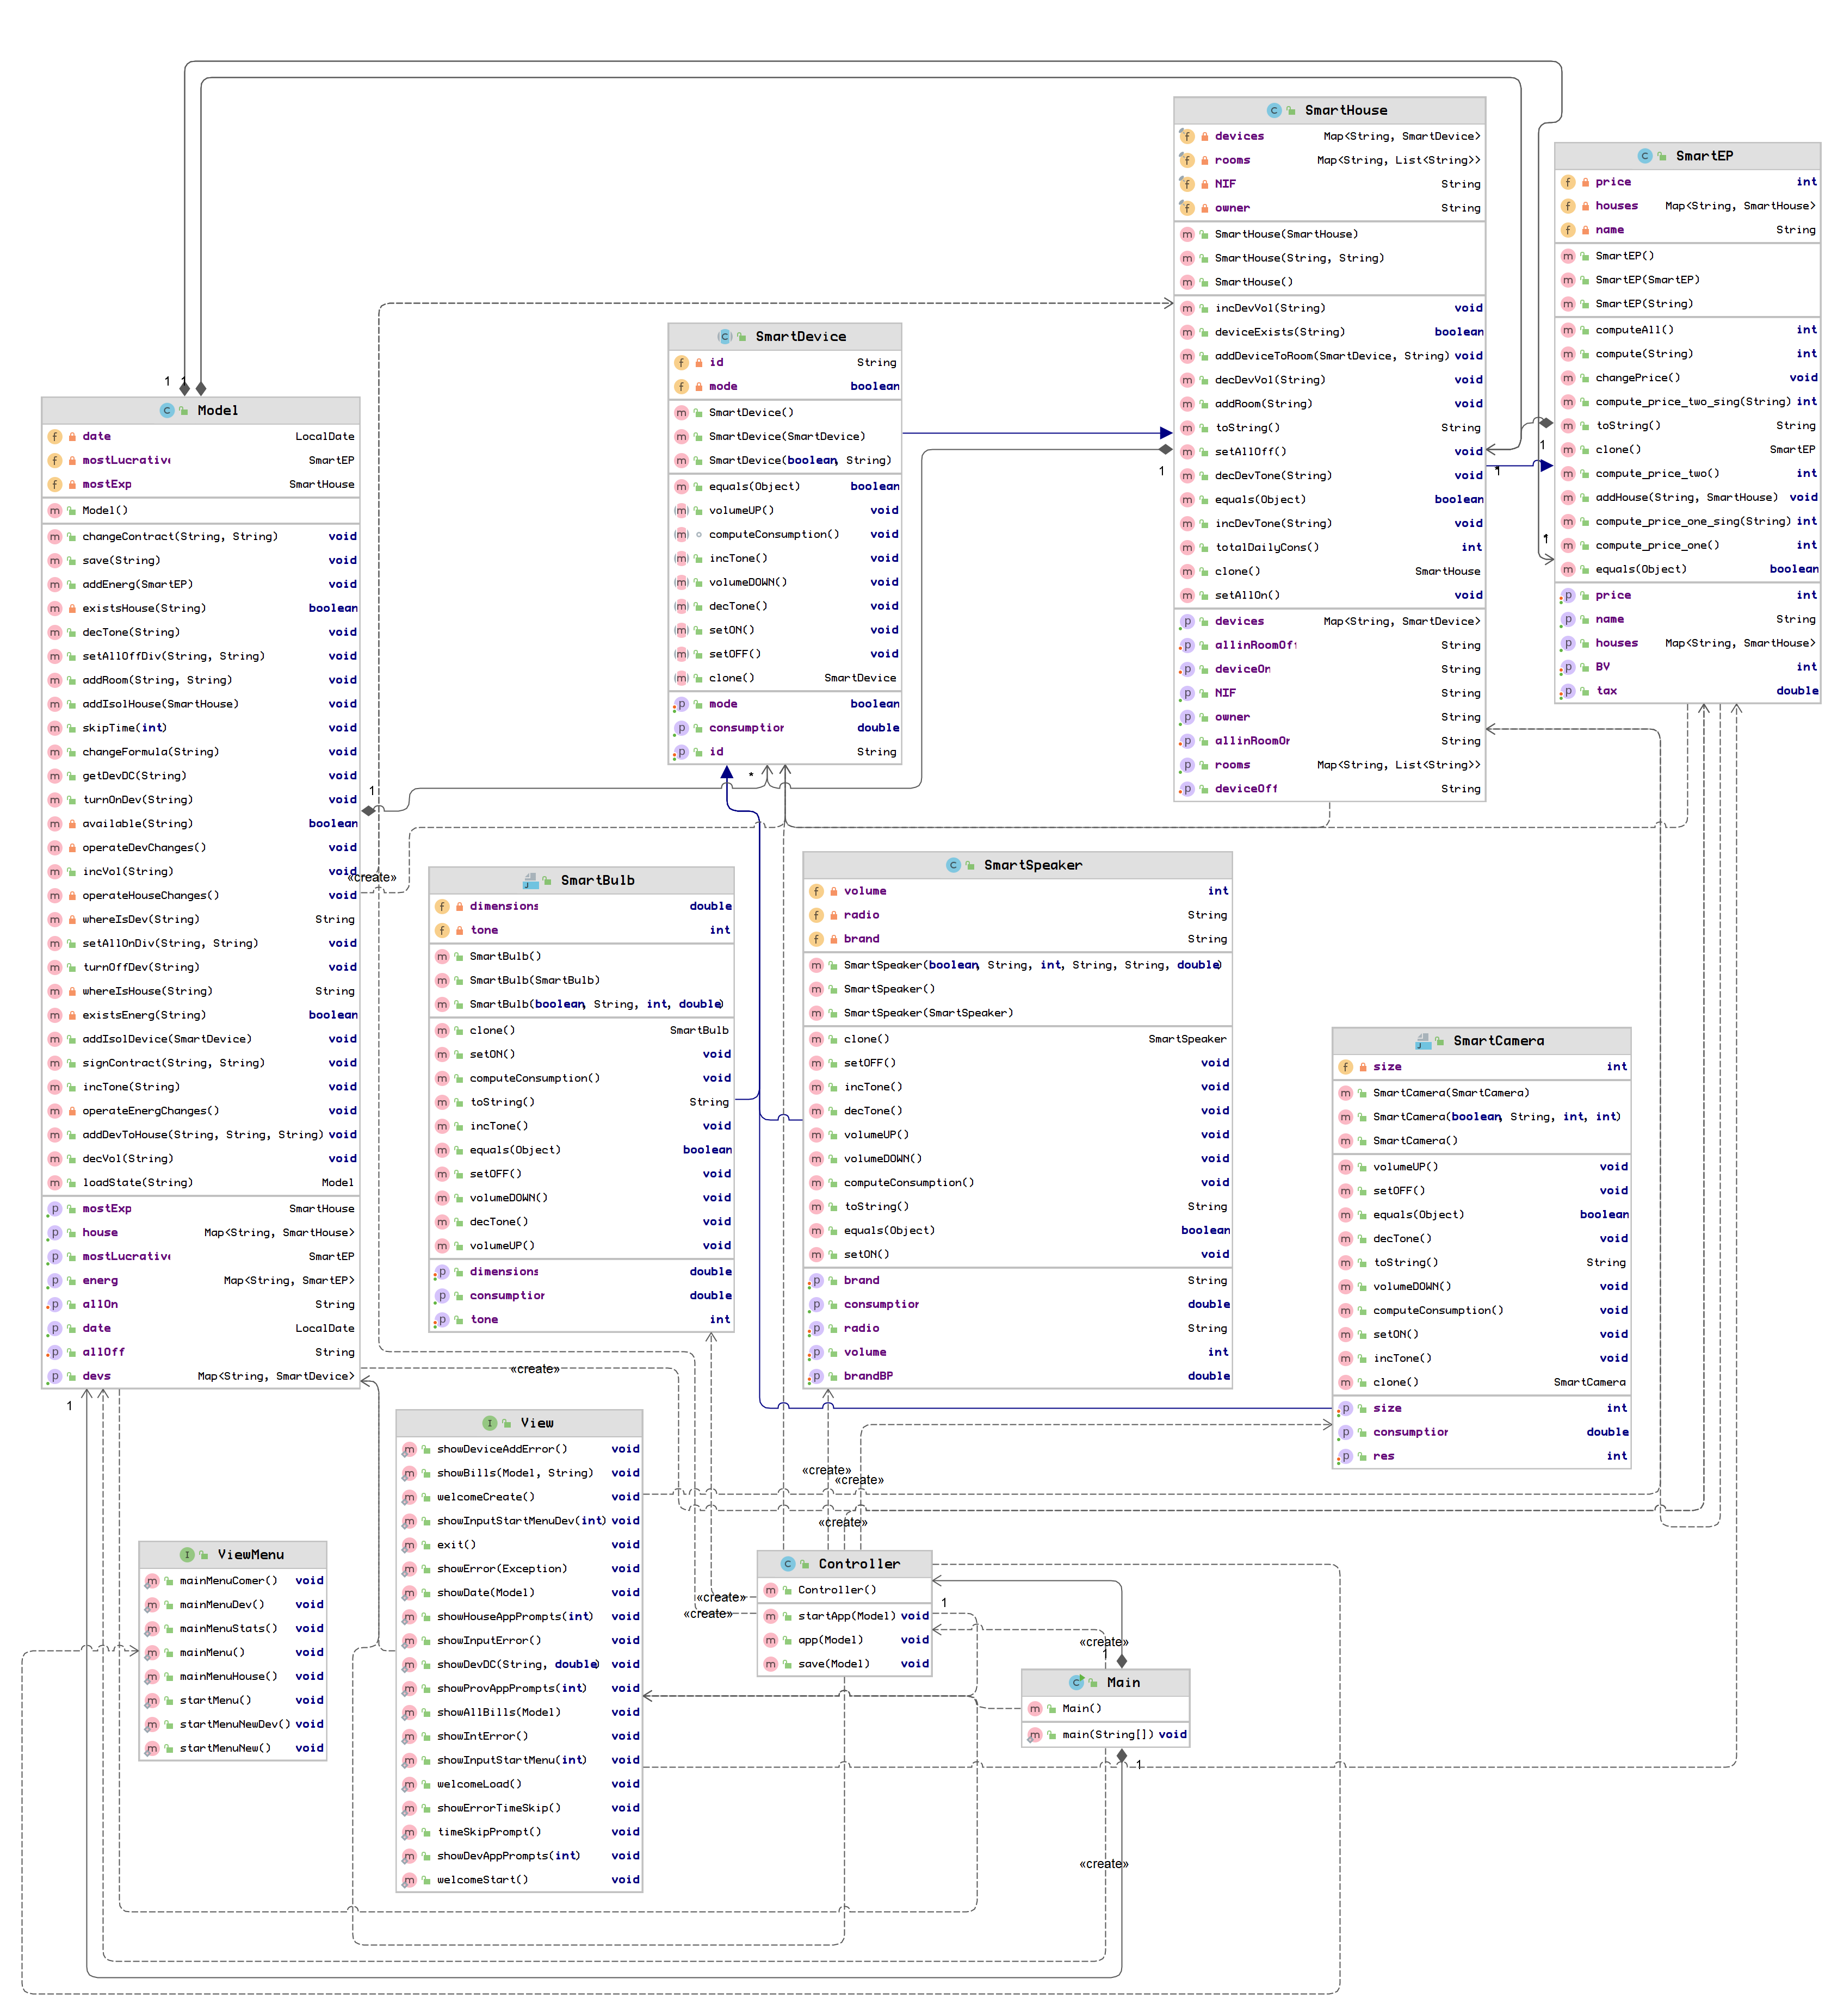
\includegraphics[width=\textwidth]{diagram_1.png}
\end{figure}
\newpage
\section{Introdução}
        Neste projeto, temos como objetivo criar uma simulação de `Casas Inteligentes'.\@
        Ora, estas usam dispositivos inteligentes que têm certas regras que os definem. Regras essas que tornam este projeto ideal para um paradigma como
        o de Programação Orientada a Objetos.\\
        Através de encapsulamento, abstração, herança e composição, conseguimos realizar este projeto, assegurando a implementação devida de POO.\@
        \\ Neste Projeto, foi utilizada a arquitetura típica de MVC (Model-View-Controller), que consiste de dividir as tarefas do programa em classes diferentes.\@
        i.e. O Model trata de gerir dos dados em memoria, o View trata da User Interface, o Controller gere a logica do programa.\@
\section{Model}
        Conforme foi explicado na introdução, o Model é a classe que trata da memória e da gestao de dados em memória, isto é, qualquer estrutura de dados,
        ou manipulação de uma estrutura de dados é feita nesta secção da arquitetura.
\subsection{Classes Base}
        De modo a implementar a tal `simulação' é necessário ter classes `base', nomeadamente as dos SmartDevices, SmartHouses e SmartEP.\@
\subsubsection{SmartDevices}
        SmartDevices são dispositivos que podem ser ligados ou desligados e têm um identificador único, no entanto, podem ser divididos em três tipos:
        SmartBulbs; SmartSpeakers e SmartCameras.
        Assim, o melhor modo de realizar esta tarefa foi claramente através do uso de uma classe Abstrata extendida pelas previamente mencionadas.
\subsubsection{SmartHouse}
        Uma SmartHouse é uma casa com dono e com uma coleção de SmartDevices, no caso deste projeto, essa coleção foi implementada através de um Map.
        De modo a garantir encapsulamento, estes são implementados através de composição.
\subsubsection{Fornecedor de Energia}
        Um fornecedor de energia é uma coleção de Casas, equipada com valores de impostos e de formulas para calcular preço por KWh.\@ 
        Fornecedores de energia também têm nome de empresa de modo a conseguir empresas armazenar num HashMap.
        De modo a colecionar estas casas, novamente, é utilizada composição.
\section{View}
        O View é a secção da arquitetura que assegura o design e a estética do Programa, sendo assim, neste projeto decidimos implementar duas interfaces, que,
        em conjunto definem o View. \\
        Estas interfaces tratam de imprimir no ecran toda a informação necessária para o utilizador conseguir correr o programa, desde menus a erros ou prompts.
\section{Controller}
        O Controller é onde o programa em si corre, tratando de invocar os métodos de View e de Model, servindo, assim, como intermediario entre estas duas secções.
\section{Simulador e Decisões de Grupo}
\subsection{Criação de uma Sessão}
        Embora uma implementação `estranha', isto é, no sentido de não ser exatamente o que se imaginaria, o modo de criar uma sessão é
        através de criar objetos até finalmente todas as casas terem assinado um contrato e, de seguida, escolher a opção de proceder no tempo. \\
        Ora, primeiramente, é necessário criar os objetos necessários, por qualquer ordem, no entanto para adicionar um objeto a uma casa é necessário: um,
        a casa existir, dois, a casa ainda não ter um contrato assinado, e três, a casa ter divisões, nomeadamente aquela qual o utilizador pretende adicionar a.\@
        Isto resulta num modo de criação sequencial e fácil de acompanhar, apesar da necessidade da casa não ter contratos assinados. \@ Ainda assim continua a ser mais acessível
        do que qualquer outro modo que tentamos implementar.
\subsection{Carregar/Guardar uma Sessão}
        Através de FileOutputStreams e FileInputStreams e do uso de MVC, é possível guardar e carregar seguramente o estado da sessão em curso.
        Isto pois, toda a informação relevante está armazenada inteiramente no Model, sendo assim é apenas necessário escrever para um ficheiro binário o
        conteúdo da classe Model. Tornando o uso de sessões anteriores não só viável mas incrivelmente eficiente e acessível para o utilizador.
\subsection{Simular a passagem de tempo, estatisticas e alterar estados}
        De modo a realizar a componente mais importante da simulação: a passagem do tempo,
        foi utilizado o package `LocalDate', fazendo uso do metodo plusDays.
        \\ Através desta funcionalidade tambem a conseguimos aproveitar para efetuar as alterações que não podem ser feitas de modo imediato,
        seja porque precisam de pelo menos um dia para efetuar, ou porque só podem ocorrer no próximo ciclo de faturação, assim através de
        uma estrutura de dados auxiliar, conseguimos efetuar essas alterações, sempre respeitando composição e encapsulamento.
        \\ Para além destas alterações, certas estatisticas são dependentes de faturações, daí ser essencial quando a passagem do tempo ocorre,
        verificar se estamos no primeiro dia do mês (por convenção de grupo, dia de faturação), calcular as estatisticas previstas para a realização do projeto.

\newpage
\section{Conclusão}
        Em suma, neste projeto prático tivemos que enfrentar diretamente as formas de programar no paradigma POO e de aplicar
        de forma inteligente e calculada a matéria que foi lecionada nas aulas teóricas e teórico práticas, acabando, ainda assim, por ser um trabalho custoso
        e de exigência acrescida. \\ \\
        Com este projeto, foi possível consolidar mais aprofundadamente os axiomas do paradigma, nomeadamente herança e encapsulamento, e aprofundar no
        conhecimento sobre a arquitetura usada na implementação do programa, nomeadamente MVC.\@ \\ \\
        Concluindo, embora trabalhoso este projeto foi essencial para a compreensão da matéria lecionada nesta UC.\@
\end{document}
